\section{Felhasználói követelmények}

A Sapi3D alkalmazás web alapú, ezért mindenki számára elérhető.
A fő célja, hogy egy 3D modellként jelenítse meg a Sapientia EMTE Marosvásárhely-i karának a főépületét, illetve ennek fontosabb helyeit, mint pl. tanszékek, titkárság stb. A rendszer fontosabb funkcionalitásait és az ezeket igénybe vevő szerepköröket a \ref{fig:UseCase} ábra szemlélteti.

Az alkalmazás eléréséhez, használatához egyetlen feltételnek kell eleget tenni, amely az internet kapcsolat megvalósítása lenne. Tekintsük meg a \ref{fig:UseCase} ábrát amely bemutatja a rendszert, amit három különböző felhasználó vehet igénybe: Visitor, User és Admin, az utóbbi kettőhöz bejelentkezés szükséges.

Visitor (látogató), amelynek lehetősége van megtekinteni az elkészített weboldalt, igénybe veheti a "vigyél el" opciót és nem utolsó sorban saját kezűleg is végig tud menni az egyetem 3D modelljén. Vannak olyan Visitor-ok akik betudnak jelentkezni, így átalakulnak User-ré. A User az aki felelős az alkalmazás karbantartásáért. A karbantartás alatt kell érteni azt, hogy az oldalon megjelenő információk napra készek legyenek. Az Admin felhasználó az, akinek a rendszerben van a legnagyobb felelőssége. Ő felel azért, hogy mely Visitorok kaphatnak engedélyt a bejelentkezéshez. Ez mellett az ő hatáskörébe tartozik, hogy ki lesz kitörölve a rendszerből.
\begin{figure}[H]
	\centering
	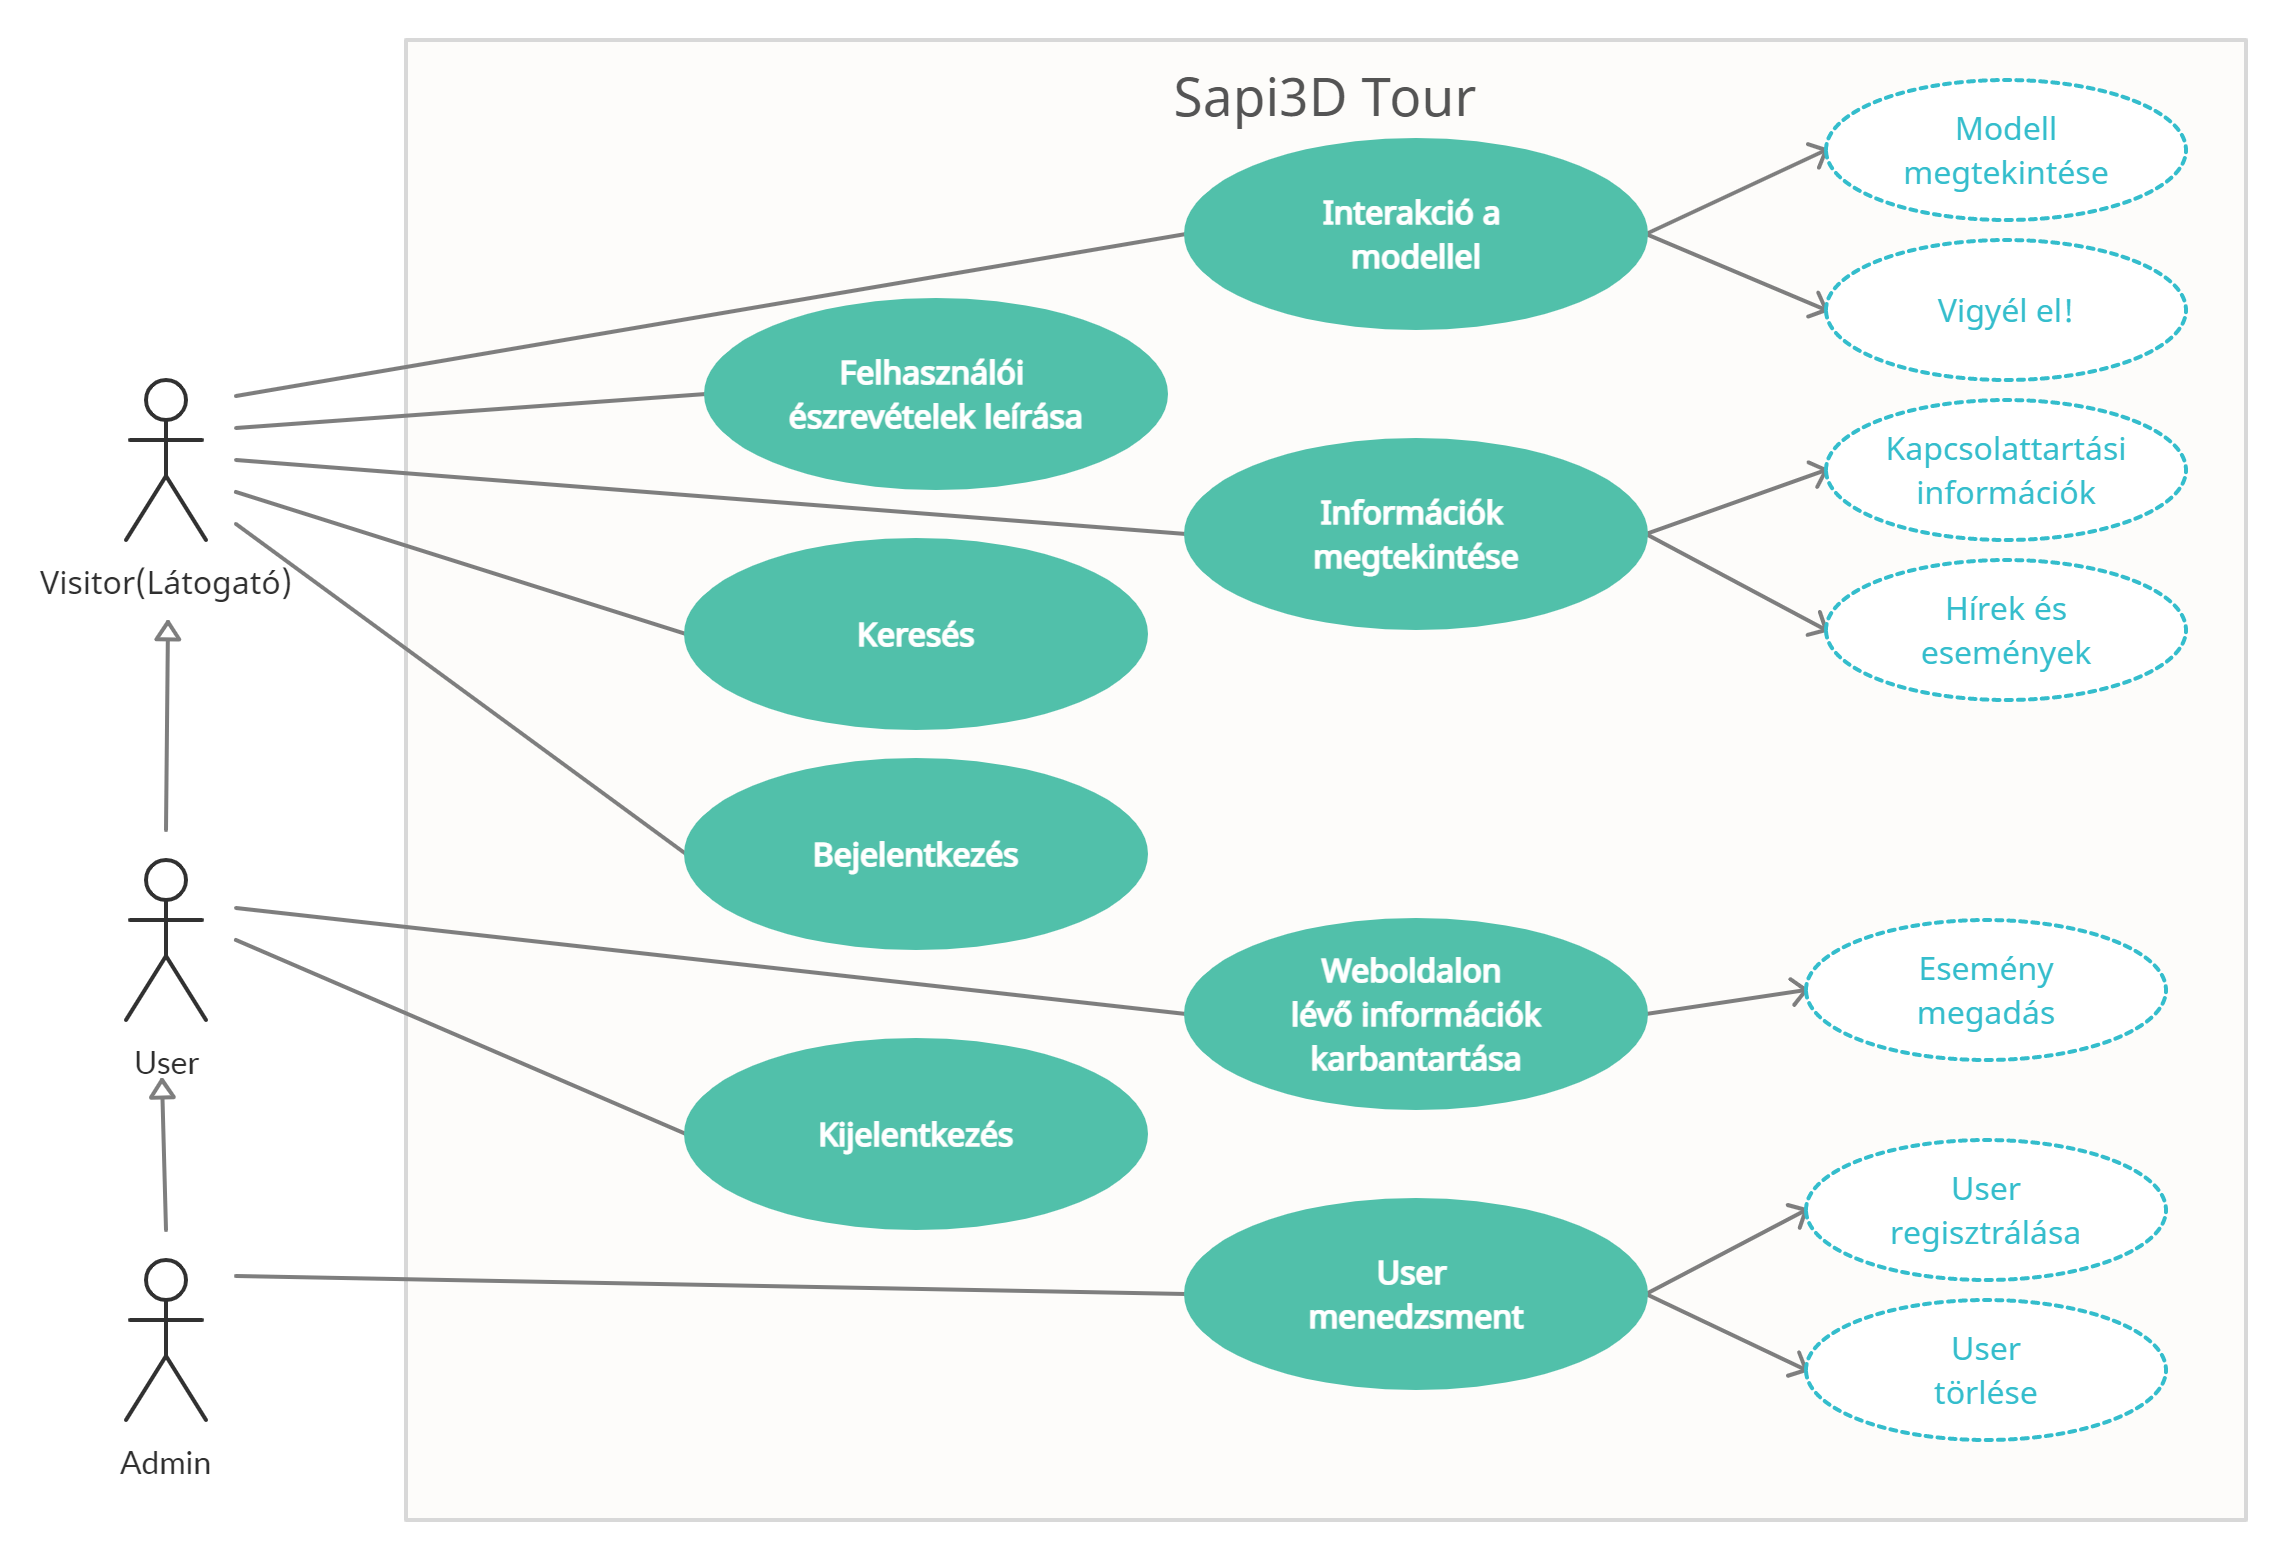
\includegraphics[width=1\linewidth]{figures/images/Sapi3dTourUseCase.png}
	\caption[A rendszer használati eset diagramja]{\textit{A rendszer használati eset diagramja}}
	\label{fig:UseCase}
\end{figure}

Bármely felhasználó, aki egy böngészőből megnyitja az oldalt, a Visitor kategóriába kerül. Ez a fajta felhasználó megtekintheti a 3D modellt, körbe sétálhatja és el tud jutni pl.titkárságra. Amint megnyílt az oldal rögtön látható az egyetemről készített modell. Ezen a modellen tud nézelődni, esetleg körbe is tudja járni, vagy adott helységekre el is tud jutni (például: titkárság, adott tanszék). Ezen kívül lehetősége van információk, elérhetőségek, események részleteinek elolvasására is. Minden Visitor ugyan akkor leírhatja saját véleményét, meglátásait az oldallal kapcsolatban is. A fent említett műveletek elvégzéséhez nem kell sem bejelentkezés, sem regisztráció.

A bejelentkezéshes szükséges megadni egy már regisztrált e-mail címet és egy már hitelesített jelszót is. A User engedélyezése nem regszitráció alapján történik, hanem az admin joggal rendelkezők osztják ki, mivel a rendszer úgy van megtervezve, hogy nincs regisztráció, hanem csak egy Admin tudja beregisztrálni az új User-eket. A regisztráció azért történik így, mert az egyetemen csak bizonyos személyeket lehet erre kinevezni, különben bárki invalid adatokkal tudná ellátni az oldalt. Egy User képes különböző műveletek elvégzésére, mint például: eseményeket megadni, az egyetemmel kapcsolatos információkat megadni, módosítani. Ezeken kívül a Usereknek lehetősége van a kijelentkezésre is.

Az Admin nem csak a Userek regisztrálásával kell foglalkozzon, hanem azoknak a törlésével is. Ezek mellett foglalkozik a teljes adatbázis menedzselésével és a rendszer újraindításával is.